%%%%%%%%%%%%%%%%%%%%%%%%%%%%%%%%%%%%%%%%%
% Large Colored Title Article
% LaTeX Template
% Version 1.1 (25/11/12)
%
% This template has been downloaded from:
% http://www.LaTeXTemplates.com
%
% Original author:
% Frits Wenneker (http://www.howtotex.com)
%
% Modified by:
% Julian Kirsch
%
% License:
% CC BY-NC-SA 3.0 (http://creativecommons.org/licenses/by-nc-sa/3.0/)
%
%%%%%%%%%%%%%%%%%%%%%%%%%%%%%%%%%%%%%%%%%

%----------------------------------------------------------------------------------------
%	PACKAGES AND OTHER DOCUMENT CONFIGURATIONS
%----------------------------------------------------------------------------------------

\documentclass[DIV=calc, paper=a4, fontsize=11pt, twocolumn]{scrartcl}

\usepackage{lipsum}
\usepackage[english]{babel}
\usepackage{microtype}
\usepackage[T1]{fontenc}
\usepackage{amsmath,amsfonts,amsthm}
\usepackage{booktabs}
\usepackage{sectsty}
\usepackage{url}
\usepackage{listings}
\usepackage[usenames,dvipsnames]{xcolor}
\usepackage[font=small,format=plain,labelfont=bf,up,textfont=it,up]{caption}

\usepackage{fancyhdr}
\usepackage{lastpage}

% ------------- neu:
\usepackage{pgf,tikz}
\usepackage{xspace}
%\usepackage{mips}
\usepackage{soul}

\graphicspath{{images/}}


% -------------- highlight bullshit:
\usepackage{lstlinebgrd}



% -------------- custom commands: ---------------
\newcommand{\sse}{S\textsuperscript{2}E\xspace}
\newcommand{\app}{\textit{SuperTaxCalcPro}\xspace}

%todo anfang
  \newcommand{\todo}[1]{
  % Add to todo list
  \addcontentsline{tdo}{todo}{\protect{#1}}
  %
  \begin{tikzpicture}[remember picture, baseline=-0.35ex]
      \node [coordinate] (inText) {};
  \end{tikzpicture}
  %
  % Make the margin par
  \marginpar{
      \begin{tikzpicture}[remember picture]
          \definecolor{orange}{rgb}{1,0.5,0}
   
          \draw node[draw=black, fill=orange, text width = 0.2cm, text height = 0.1cm] (inNote)
                   {#1};
      \end{tikzpicture}
  }
  %
  \begin{tikzpicture}[remember picture, overlay]
      \draw[draw = orange, thick]
          ([yshift=-0.2cm] inText)
              -| ([xshift=-0.2cm] inNote.west)
              -| (inNote.west);
  \end{tikzpicture}
  %
  }
% todo ende


\sloppy
\hbadness 10000
\renewcommand*\rmdefault{ppl}\normalfont\upshape
\renewcommand{\topfraction}{0.85}
\renewcommand{\textfraction}{0.1}
\renewcommand{\floatpagefraction}{0.75}
\renewcommand{\UrlFont}{\small\tt}
\allsectionsfont{\color{tumblue}\usefont{OT1}{phv}{b}{n}}

\usepackage[osf, sc]{mathpazo}
\usepackage{helvet}

\definecolor{tumblue}{RGB}{0,101,189}

% https://en.wikibooks.org/wiki/LaTeX/Source_Code_Listings
\lstset{
  numbers=left,
  numberstyle=\tiny\color{gray},
  stepnumber=1,
  numbersep=5pt,
  showspaces=false,
  showstringspaces=false,
  showtabs=false,
  frame=single,
  rulecolor=\color{black},
  tabsize=8,
  captionpos=b,
  breaklines=true,
  breakatwhitespace=false,
  language=C,
  keywordstyle=\bfseries\color{OliveGreen},
  commentstyle=\itshape\color{Mahogany},
  stringstyle=\color{BrickRed},
  keywordstyle=[2]{\color{Cyan}},
  escapechar=ß,
  xleftmargin=8pt,
  xrightmargin=3pt,
  basicstyle=\scriptsize,
  morekeywords={u32, __u32, __be32, __le32,
  		u16, __u16, __be16, __le16,
	        u8,  __u8,  __be8,  __le8,
	        size_t, ssize_t}
}

% https://tex.stackexchange.com/questions/51645/
%  x86-64-assembler-language-dialect-for-the-listings-package
\lstdefinelanguage
   [x86_64]{Assembler}
   [x86masm]{Assembler}
   % with these extra keywords:
   {morekeywords={CDQE, CQO, CMPSQ, CMPXCHG16B, JRCXZ, LODSQ, MOVSXD,
                  POPFQ, PUSHFQ, SCASQ, STOSQ, IRETQ, RDTSCP, SWAPGS,
                  rax, rdx, rcx, rbx, rsi, rdi, rsp, rbp,
                  r8, r8d, r8w, r8b, r9, r9d, r9w, r9b}}

\usepackage{lettrine}
\newcommand{\initial}[1]{
\lettrine[lines=3,lhang=0.3,nindent=0em]{
\color{tumblue}
{\textsf{#1}}}{}}



%----------------------------------------------------------------------------------------
%	TITLE SECTION
%----------------------------------------------------------------------------------------

\usepackage{titling}
\newcommand{\HorRule}{\color{tumblue} \rule{\linewidth}{1pt}}

\pretitle{\thispagestyle{noheadings}\vspace{-30pt}
  \begin{flushleft} \HorRule \fontsize{30}{40} \usefont{OT1}{phv}{b}{n} \color{tumblue} \selectfont}

\title{Selective Symbolic Execution}
% \\ \large Analysis of user space binaries using the \sse platform}

\posttitle{\par\end{flushleft}\vskip 0.5em}

\preauthor{\begin{flushleft}\large \lineskip 0.5em \usefont{OT1}{phv}{b}{sl}
  \color{tumblue}}

% Please leave this as it is for the 1st draft as our "peer-review"
% is supposed to take place anonymously (like in real life)
\author{Anonymous}

\postauthor{\footnotesize \usefont{OT1}{phv}{m}{sl} \color{Black} % Configuration for the institution name
, Technische Universit\"at M\"unchen

\par\end{flushleft}\HorRule}
\date{}

%----------------------------------------------------------------------------------------
\makeatletter
\let\docauthor\@author
\makeatother
\makeatletter
\let\doctitle\@title
\makeatother


\fancypagestyle{headings}{
  \lhead{}
  \chead{}
  \rhead{\usefont{OT1}{phv}{m}{sc}\footnotesize \doctitle }

  % Footers
  \lfoot{\usefont{OT1}{phv}{m}{sc}\footnotesize \docauthor }
  \cfoot{}
  \rfoot{\usefont{OT1}{phv}{m}{sc}\footnotesize Page \thepage\ of \pageref{LastPage}}

  \renewcommand{\headrulewidth}{0.4pt}
  \renewcommand{\footrulewidth}{0.4pt}
}

\fancypagestyle{plain}{
  \fancyhf{}

  % Footers
  \lfoot{\usefont{OT1}{phv}{m}{sc}\footnotesize \docauthor }
  \cfoot{}
  \rfoot{\usefont{OT1}{phv}{m}{sc}\footnotesize Page \thepage\ of \pageref{LastPage}}

  \renewcommand{\headrulewidth}{0.0pt}
  \renewcommand{\footrulewidth}{0.4pt}
}
\lfoot{\usefont{OT1}{phv}{m}{sc}\footnotesize \docauthor }
\cfoot{}
\rfoot{\usefont{OT1}{phv}{m}{sc}\footnotesize Page \thepage\ of \pageref{LastPage}}


\begin{document}


% Stop whining, \maketitle
\newcommand{\undefinedpagestyle}{}
\maketitle
\pagestyle{headings}

%----------------------------------------------------------------------------------------
%	ABSTRACT
%----------------------------------------------------------------------------------------

% The first character should be within \initial{}
\initial{T}\textbf{his paper describes the exemplary application of selective symbolic execution techniques for the analysis of a binary file in user mode.
Goal of this study is to search the binary for possible privacy issues like unwanted leakage of personal data.
Investigation will be done using \sse, a powerful platform for selective symbolic execution of large software systems.
}

%----------------------------------------------------------------------------------------
%	ARTICLE CONTENTS
%----------------------------------------------------------------------------------------

\bigskip

\section{Introduction}

% use cases (sel symb exe paper kap 2) hier hinein?

Frequently developers need to understand software systems.
In a very simple case they just analyse their own code or test the interaction of own programs with other components or with the surrounding environment in general.
Testing self-written programs conceptually permits the application of the whole arsenal of analysis techniques.


Things become interesting when analysis has to be performed without access to source code or documentation.
Scenarios for this situation include the need to check proprietary third party software for interoperability on existing servers, performance, unwanted side effects, and much more.
Security-critical environments additionally require reliable guarantees of the benignity of all employed software.


One mighty solution for such system analysis is the \sse platform developed at the Swiss Federal Institute of Technology in Lausanne (EPFL) \cite{chip11s2e}.
Its goal is to provide a tool set for rapid development of analysis tools like performance profilers, bug finders, reverse engineering solutions and the like \cite{chip12s2e}.
\sse combines several key characteristics:

\medskip
1.) The ability to explore entire \textit{families of execution paths} helps to obtain reliable information about the target system.
Abstracting from single-path exploration to sets of execution paths which share specific properties is vital for predictive analyses.
This technique can for example prove the non-existence of critical corner cases which might be overlooked by other testing strategies.
% ...and hence provides more reliable results.
%Particularly for predictive tasks the analysis of sets of execution paths which share specific properies
%This is often necessary for predictive analyses, where classical single-path exploration techniques fail to provide reliable results.

\medskip
2.) \textit{In-vivo analysis}, meaning the analysis of a program within its real-world environment (libraries, kernel, drivers, etc.), facilitates extremely realistic and accurate results.

\medskip
3.) Working directly on \textit{binaries} further increases the degree of realism in system analyses, as it allows to include closed source modules into the investigation.

\bigskip

As an exemplary showcase for the power of the \sse platform and its underlying concepts this paper will perform a thorough analysis of a binary file in user mode.
The scenario assumes that this program was found somewhere in the internet and claims to be a useful freeware tool.
\sse shall help to investigate whether the binary compromises the user's privacy, for instance by leaking private data to the internet.


%What I do is bla...
%...justify the choice of \sse as platform for system analysis.\todo{?}

\bigskip

Chapter \ref{sec:s2e} explains the theoretical concepts of selective symbolic execution.
Chapter \ref{sec:platform} then introduces \sse, the platform which builds upon all techniques described before.
Coming to the practical part, chapter \ref{sec:proj} lays out the concrete analysis scenario and formulates research questions.
Chapter \ref{sec:impl} describes how \sse can be applied in this scenario, followed by an explanation of \sse results in chapter \ref{sec:ana}.
Possible further research related to this topic is mentioned in chapter \ref{sec:outlook}, together with some selected related work in chapter \ref{sec:rel_work}.
Finally, chapter \ref{sec:conclusion} summarises and concludes this paper.

%\newpage
\iffalse
§1	Introduction (Motivation)
		> Motivation, warum es einen Bedarf für etwas wie S2E gibt
		> Kurze Vorschau, was man damit Tolles machen kann
			-> Pfadanalyse -> Prediction of system behaviour
			-> Analyse in natürlicher Umgebung -> “in-vivo”

§2	Selective Symbolic Execution
		> Theorie-Teil
		> Was ist Symbolic Execution?
		> Was kann Selective Symbolic Execution besser?
			(Concrete -> symbolic transition usw.)
		> Konsistenzmodelle (wird hier evtl. schwierig, das richtige Maß 
			zu finden, um die Sache auf wenig Platz zu verstehen)

§3	The S2E Platform
		> Architektur
		> Funktionsweise
		> Selektoren + Analysatoren

§4	Project idea: explore privacy issues in a sample binary
		> Plan darlegen: Programme könnten unerwünscht Infos preisgeben.
		> Daher: Eigenes kleines Programm, das … macht.

§5 	Implementation (of the test case using S2E)
		> Vorgehen
		> Verwendete Konsistenzmodelle
		> Arbeitsweise von Selektoren/Analysatoren

§6	Interpretation of S2E analysis output
		> Execution Traces
		> Gefundene Privacy-Probleme
		> Eventuell nicht gefundene Sachen
		> Probleme bei der Analyse

§7	Outlook
		> Was man sonst noch Tolles machen könnte.
		> Anwendung auf echte Malware, etc…

		> Kommt das hier zu früh? Evtl. auch in den Schlussteil...

§8	Related Work
		> Was haben andere mit S2E in ähnlicher Richtung gemacht?
		> Z.B. "Finding Trojan Message Vulnerabilities in Distributed Systems”

§9	Conclusion
		> Zusammenfassung: was habe ich gemacht?
		> Fazit: war die Sache sinnvoll und erfolgreich?
\fi







\section{Selective Symbolic Execution}\label{sec:s2e}

% - evtl. einbauen:
% ------ KLEE arbeitet auf Code -> S2E auf binaries!


% -------- symbolic execution -------- %
\textbf{Symbolic execution} is an advanced analysis technique particularly suited for automated software testing \todo{ct} and malware analysis \todo{ct}.
Instead of concrete input (7, ``string'', ...) symbolic execution uses symbolic values ($\lambda$, $\beta$, ...) when processing code.
Assignments in the program path have impacts on these symbolic values.
The integer calculation $x = x - 2$, for instance, would update the symbolic expression representing the input $x$ to $\lambda - 2$.
Conditional statements (if <condition> then ... else ...) fork program execution into two new paths.
Both paths are then constrained by an additional condition, the `then' branch with the if-condition and the `else' branch with the negated if-condition respectively.
\todo{Bild > Text}

\begin{figure}
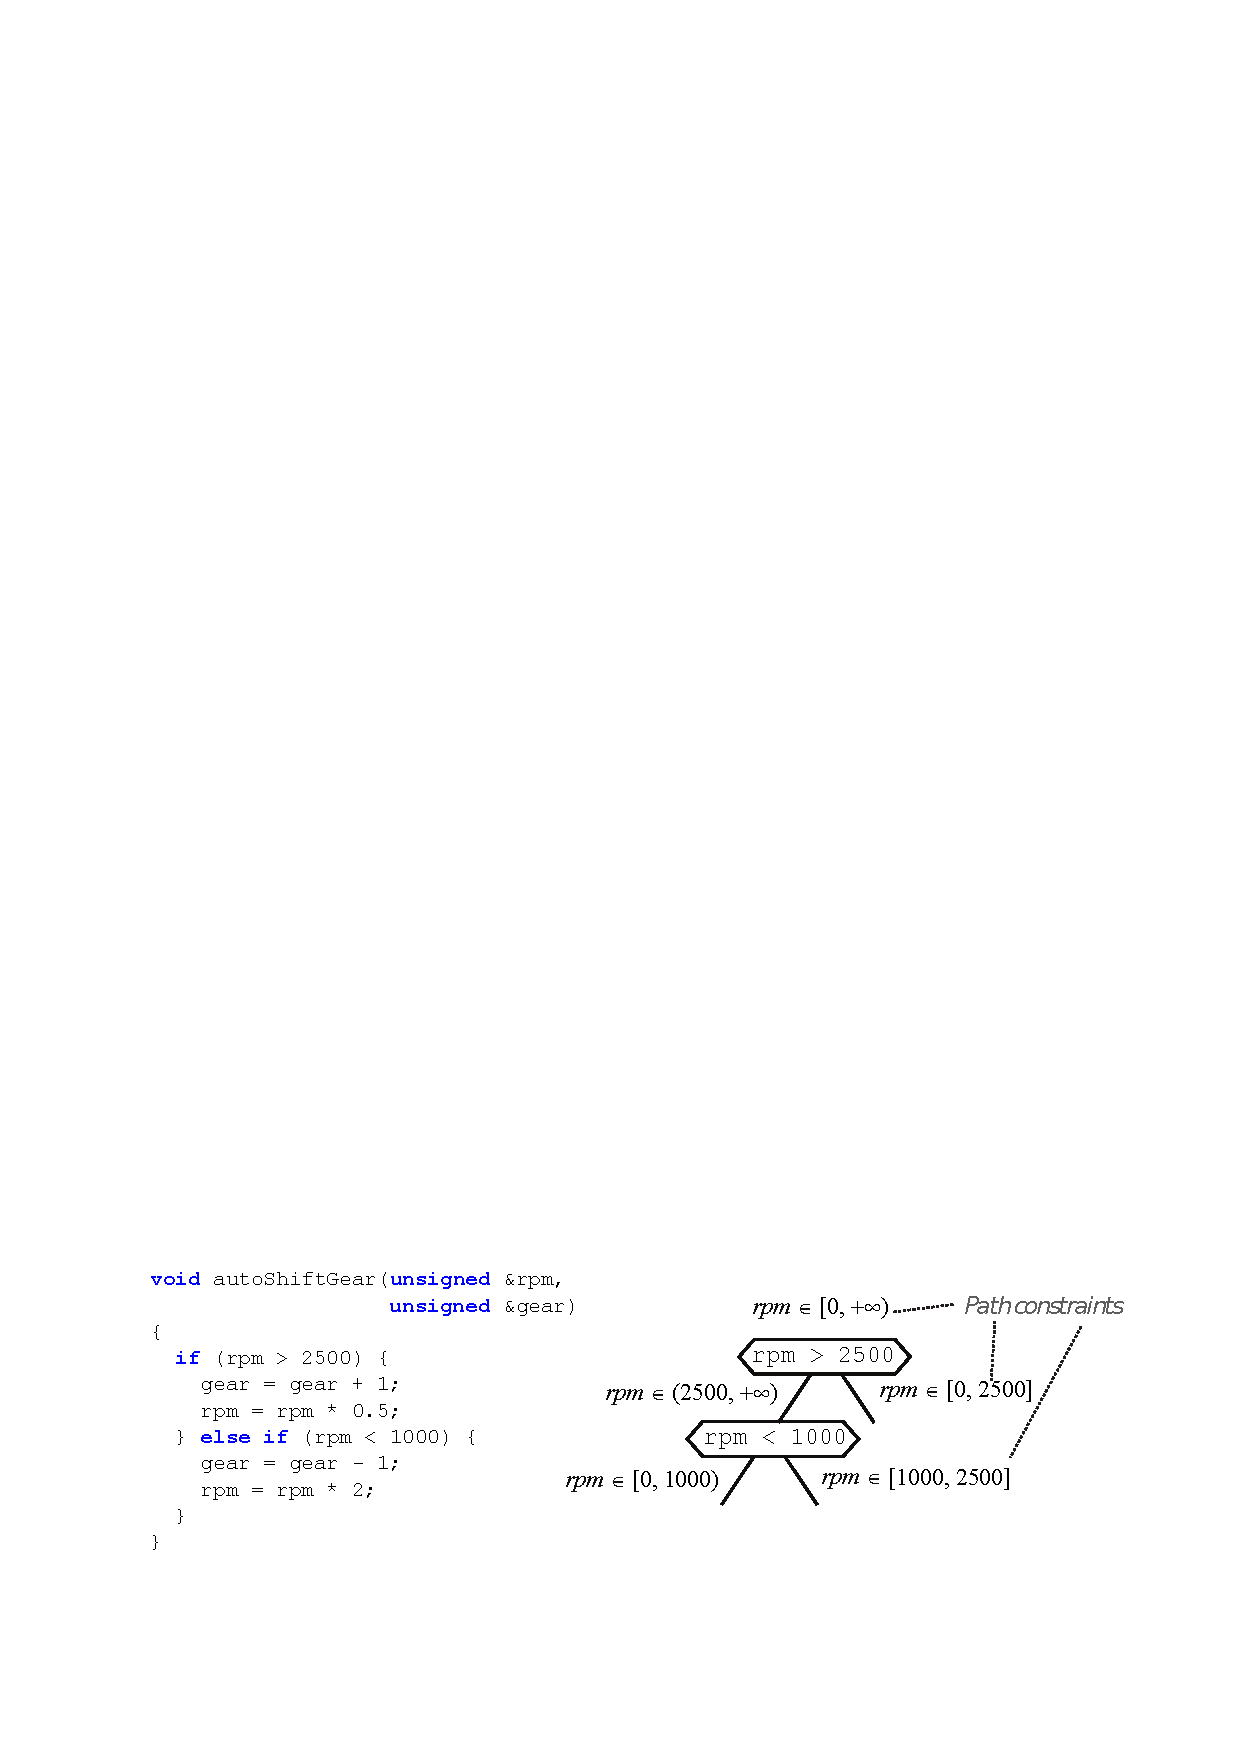
\includegraphics[width=\columnwidth]{symb_exe_2}
\caption{Execution tree with path constraints for the symbolic variable $rpm$ \cite{chip14s2e}}
\label{fig:arch}
\end{figure}

Following this procedure results in a tree-like structure of constrained symbolic expressions.
A constraint solver can now take all constraints along one execution path as input and find one concrete input (e.g., $\lambda = 5$) which would lead to the program following exactly this path.
Such results greatly alleviate writing reproducible test cases \cite{chip09sel}.

On a technical level, symbolic execution engines save state information (program memory, constraint information, ...) in a custom data structure.
Each conditional statement involving symbolic values results in a $fork$ of the program state.
The two newly created branches are completely independent and can therefore be processed in parallel.

% -------path explosion
But the exponential growth of conditionals soon reveals scaling problems of this forking strategy.
Despite heavy research on optimisations mitigating this \textit{path explosion} problem \todo{ct} only relatively small programs ($\cong$ thousands of lines of code) can be analysed symbolically \cite{chip09sel}.

% -------interaction with env
%In addition to the path explosion problem, classical symbolic execution ... interaction with the environment...
Additionally, symbolic execution faces problems when the program under analysis \textit{interacts with its environment}.
If it calls a system library like $libc$, in theory the whole system stack including invoked libraries, operating system and drivers would have to be executed symbolically.
Considering the path explosion problem mentioned before, the resulting complexity makes such a profound analysis hardly feasible.

% --------standard sol
One way to solve this problem is to build abstract models of the program's environment \todo{ct}.
However, due to the complexity of real-world systems, building a model of the entire system is both tedious and unnecessary - the user usually wants to analyse one single program and not the whole system \cite{chip09sel}.

\bigskip

% -------- selective symbolic execution -------- %
In order to overcome typical problems of conventional symbolic execution, Chipounov et al.~from the Swiss Federal Institute of Technology in Lausanne (EPFL) developed the concept of \textbf{selective symbolic execution} (\sse) \cite{chip09sel}.
Based on a virtual execution platform \sse gives users the illusion of running the entire system symbolically.
By limiting the scope of interest (i.e.~which parts of the system should be executed symbolically), users can effectively restrain the path explosion problem.
Program code within this defined scope is executed symbolically, whereas out-of-scope parts, which are irrelevant to the analysis, switch to concrete execution.
%One of the main contributions of the EPFL team around Chipounov is the transparent and consistent management of switching between symbolic and concrete execution modes.

% puning for scalability -> bringen?

Definition of the scope of interest (what to execute symbolically) is highly flexible.
Users may specify whole executables, code regions, or even single variables to be executed symbolically. Everything else will be treated concretely.

%This forth and back conversion -> challenge!
But since on a technical level symbolical and concrete execution are handled very differently - concrete code may run natively while symbolic instructions need to be emulated - switching back and forth these two modes is a major challenge.
Hence one of the main contributions of the EPFL team around Chipounov is the transparent and consistent management of switching between symbolic and concrete execution modes.

\todo{kill}
\cite{chip09sel}
\cite{chip11s2e}
\cite{chip12s2e}
\cite{chip14s2e}





% -------- Konsistenzmodelle -------- %

bla bla bla



%%%%%%%%%%%%%%%%%%%%%%%%%%%%%%%%%%%%%%%%%%%%%%%%%%%%%%%
\iffalse
§2	Selective Symbolic Execution
		> Theorie-Teil
		> Was ist Symbolic Execution?
		> Was kann Selective Symbolic Execution besser?
			(Concrete -> symbolic transition usw.)
		> Konsistenzmodelle (wird hier evtl. schwierig, das richtige Maß 
			zu finden, um die Sache auf wenig Platz zu verstehen)
\fi

\section{The \sse Platform}\label{sec:platform}

Based on the concepts described in the previous chapter, Chipounov and his team implemented the \sse platform, an open source framework for writing custom system analysis tools.
\sse employs the theoretical concepts of selective symbolic execution by running the system under analysis in a virtual machine and treating code within the scope of interest as symbolic.
These symbolic parts are translated into an intermediate representation (\todo{.}), while irrelevant instructions are directly passed to the host for native execution.


Technical backbone of \sse are the virtual machine hypervisor QEMU \cite{qemu, qemu05}, the symbolic execution engine KLEE \cite{klee, klee08} and the LLVM compiler infrastructure \cite{llvm, llvm04}.
Figure \ref{fig:arch} gives an overview of how these technologies are integrated into the \sse platform.
The top of the picture depicts the software stack of the guest system (=the system under analysis), which is managed by QEMU.
\sse is not restricted to user land applications, but also allows inspection on deeper levels (e.g., operating system functions).


\begin{figure}
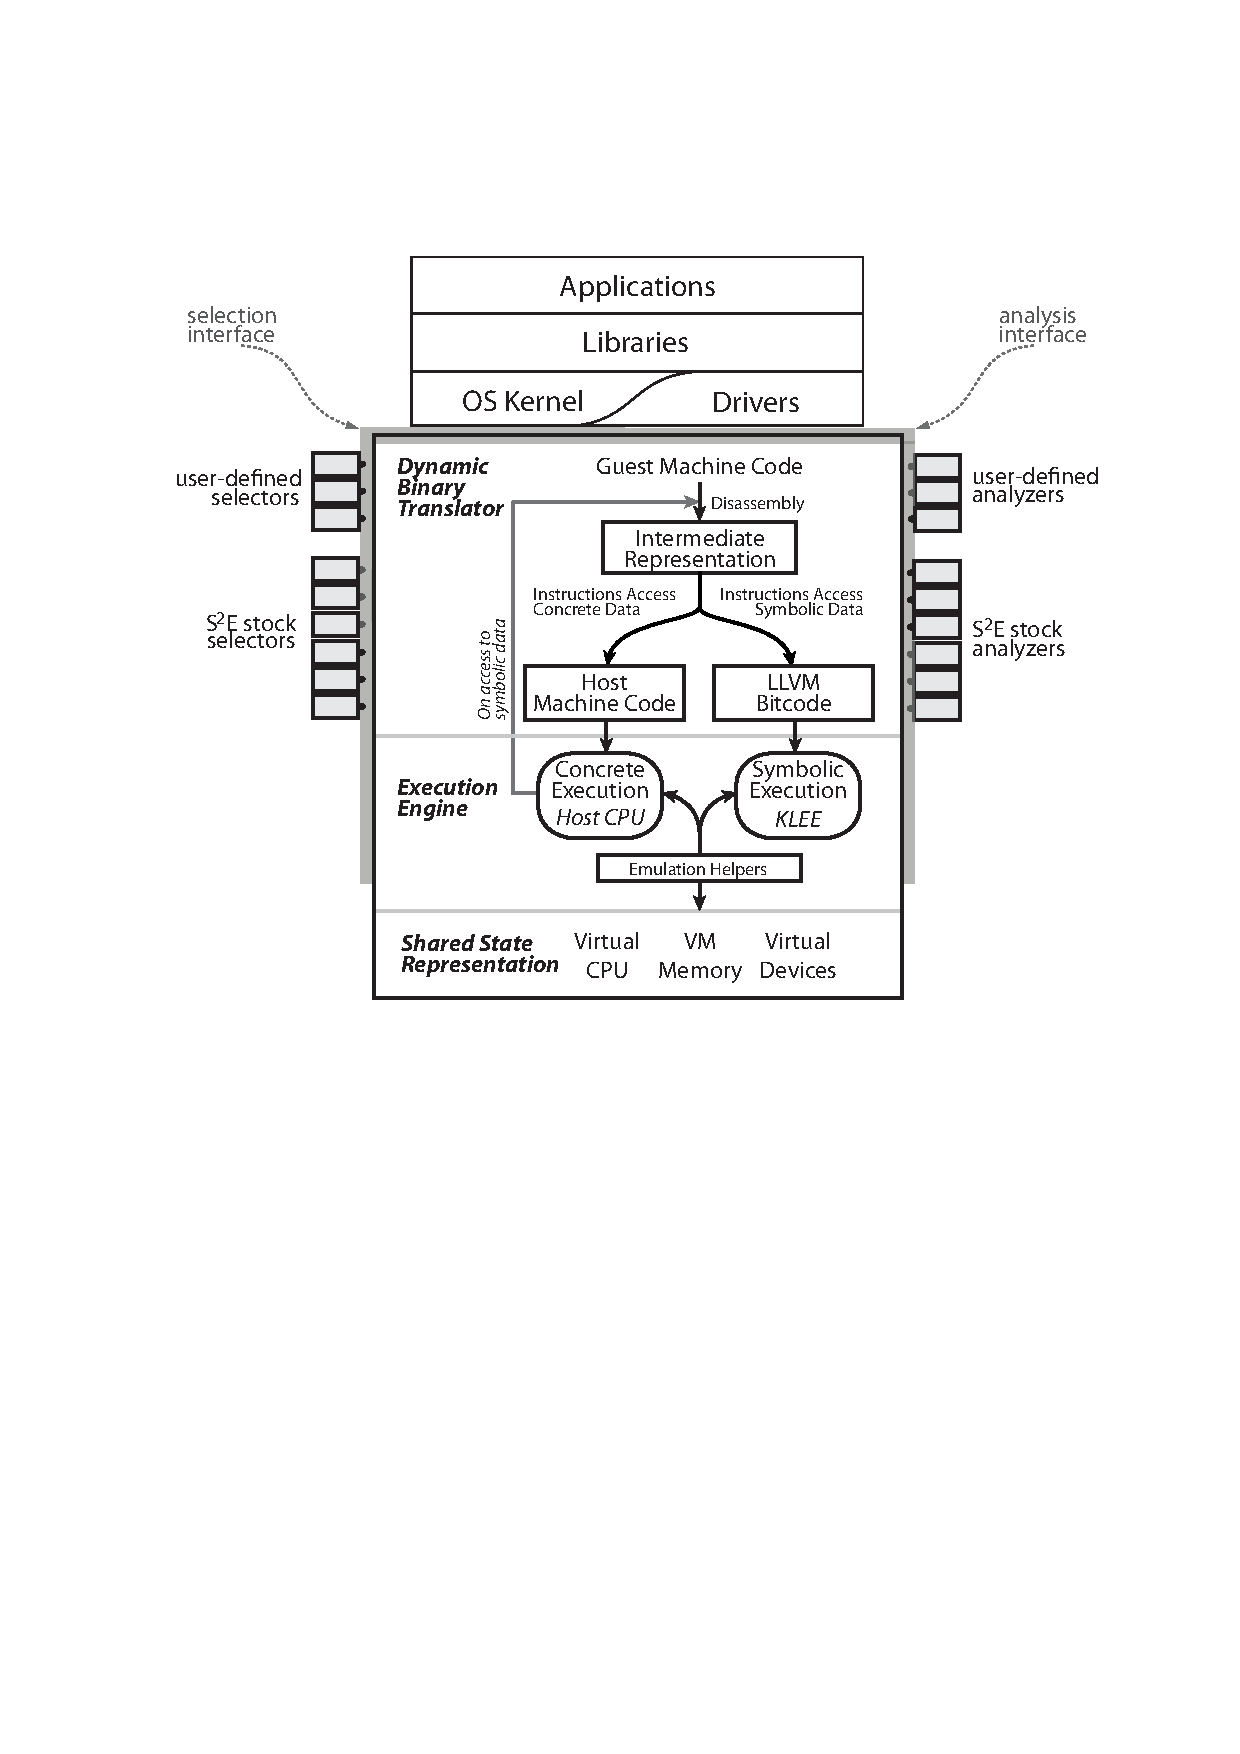
\includegraphics[width=\columnwidth]{s2e_arch}
\caption{Architecture of the \sse platform \cite{chip12s2e}}
\label{fig:arch}
\end{figure}


For easier emulation, QEMU translates machine code of the guest system into an intermediate representation, called $microoperations$.
\sse's dynamic binary translator (DBT) splits the resulting microoperations into those that need to be explored symbolically and those which may run concretely.
All concrete microoperations are directly converted into host instructions.
Symbolic expressions, on the other hand, are prepared for being executed on the KLEE engine.
This requires microoperations to be translated into the LLVM intermediate representation, called LLVM Bitcode in figure \ref{fig:arch}.

\sse's execution engine, which is an extension to QEMU's execution engine, now manages the operation of the platform.
In an endless loop it asks the DBT for new guest code.
Depending on the result, instructions can either be run straight on the host system or are fed into the KLEE symbolic execution engine.
% --- - --- - Emulation Helpers bringen?

In order to keep the mix of symbolic and concrete execution consistent, \sse stores state (VM CPU, memory, ...) centrally, by consolidating QEMU and KLEE data structures and managing them in a single machine state representation.
% - --- - - - Effizienz bringen?


Users work with \sse by writing selection and analysis plugins or by simply configuring \sse's standard plugins according to their needs.
Plugins subscribe to system-wide events (e.g., $onInstrExecution$) and can perform logging/monitoring tasks or even manipulate the system state.

Configuration usually starts with defining what parts of the system to explore symbolically.
This can for example be done with \sse's selection plugin $CodeSelector$, which restricts symbolic execution to a specified module or code region.

Standard analysis plugins allow users to find bugs ($WinBugCheck$), monitor memory ($MemoryChecker$), study performance characteristics ($PerformanceProfiler$) and much more (see \cite{chip14s2e}, p.~50).
% - ------- hier mehr?
\todo{m?}



% ---------------------------------------------------------------- %
\iffalse
§3	The S2E Platform
		> Architektur
		> Funktionsweise
		> Selektoren + Analysatoren
\fi
\section{Design Alternatives}\label{sec:alt}

\section{Implementation}\label{sec:impl}

\todo{.}Klar machen, welche Plugins ich verwendet habe! Liste.\todo{.}

As described in chapter \ref{sec:s2e}, working with \sse can be divided into a code selection and the actual analysis part.

In the \textbf{code selection phase} \sse is configured to focus on the program \app in user space only.
The whole environment will be treated as a black box.
% Possible calls into the kernel are assumed to work correctly.
Symbolic execution will only be applied inside the code of \app.

The next step is to precisely specify which variables shall be treated symbolically.
In general, as a start we want to make all user inputs symbolic.
For a closed source binary this can be done in several ways.
A command line tool can be called from a wrapper program which hands over symbolic arguments instead of concrete ones.
If user input is entered in a UI, a further code into the assembly code is necessary in order to find the memory locations where the corresponding variables are written.\todo{..}
%look for ... calls...
\sse can intercept execution of the specified memory addresses and replace them with symbolic values (state:writeMemorySymb(\ldots)).\todo{con?}
% consistency models?????

KLEE, the engine for symbolic execution, also requires some configuration.
As path search strategy this analysis uses a depth first search.
\todo{..}

\bigskip

Most logic in the \textbf{analysis part} relies on \sse's \textit{Annotations} plugin.
It allows fine monitoring and even fiddling with the execution state by annotating single instructions or functions in the program binary.

For the scenario in this paper all instructions which handle connections to the internet are of particular interest.
The C library call \textit{connect} helps to identify where the program is connecting to, and the corresponding \textit{write} and \textit{read} calls allow to find out what data is sent and received in this connection.
Memory addresses of these relevant calls can be retrieved from the assembly code.
Since all calls concerned with connecting to the internet seem to take place in a single function named \textit{send\_data}, calls to this function as a whole shall be monitored, too.

After providing \sse's \textit{Annotations} plugin with all relevant memory addresses plus a little more configuration, we can now execute code every time the program runs into one of the interesting instructions.
At this point, we will \ldots

1.) log that instruction $X$ was reached.
Together with other \sse output this information shows which execution paths run into the \textit{send\_data} method and when they do so.

2.) save information about the executed instruction in the current plugin state.
This allows to check whether there have been prior connections to the internet when the program runs into the next annotated instruction.

3.) read out parameters of the called function.
The function \textit{send\_data}, for instance, is called with one parameter, which appears to be a memory location.
Now \sse's analysis interfaces can be employed to dynamically find out what is written in the respective memory.

4.) read (or write) registers (EAX, ESP, ...).
... Check out call conventions of write, ...
%This may either be used to check the current internal state, or...

5.) switch variables (memory locations) from concrete to symbolic mode (or vice versa).
... Nice for controlling consistency models. Not used currently.

% -------------------------------------------------------------------
\begin{lstlisting}[language={[5.0]Lua}, basicstyle=\ttfamily\footnotesize, caption={Configuration of the \textit{Annotations} plugin (part). Defines the instructions to be monitored and actions to trigger upon execution of these instructions.}, label={lst:ann_def}]
pluginsConfig.Annotation = {
  annotation_write = {
    active=true,
    module="prog",
    address=0x8049523, -- write()
    instructionAnnotation="do_write",
    beforeInstruction=true,
    switchInstructionToSymbolic=false
  },
  annotation_read = {
    active=true,
    module="prog",
    address=0x804956b, -- read()
    instructionAnnotation="do_read",
    beforeInstruction=false, 
    switchInstructionToSymbolic=false
  },
  annotation_send_data = {
    active=true,
    module="prog",
    address=0x804940c, -- send_data()
    callAnnotation="call_ann",
    paramcount = 1
  }
}
\end{lstlisting}


% -------------------------------------------------------------------
\begin{lstlisting}[language={[5.0]Lua}, basicstyle=\ttfamily\footnotesize, caption={Lua function executed upon every call of the function send_data().}, label={lst:send_data}]
function call_ann (state, curPlgState)
  if curPlgState:isCall() then
    arg0 = state:readParameter(0);
    print ("Calling function with with arg0=" .. ("%x"):format(arg0));
    -- print_mem dereferences the pointer arg0 and converts the memory behind that address into a string.
    print_mem(state, curPlgState, arg0);
    -- saving info about the no. of connections in this state so far
    local no =curPlgState:getValue("no");
    if no == nil then
      no = 0
    end
    no = no + 1;
    curPlgState:setValue("no", no);
    print ("\n\tNo. of connections on this path so far: " .. no);
  else
    -- Called when the function send_data returns. The return value can be read from the EAX register.
    local eax =state:readRegister("eax");
    print("EAX: " .. ("%x"):format(eax));
  end
end
\end{lstlisting}

Figure \ref{} shows relevant parts of the assembly code. Figure \ref{} presents excerpts from the resulting analysis plugin.

\bigskip

In addition to the \textit{Annotations} plugin, analysis in this paper also employs the \textit{TestCaseGenerator}.
For each execution path, it finds concrete inputs for all symbolic variables.
Those will be printed upon termination of the path and, apart from helping to understand the program, may serve as input for further testing.



\iffalse
§5 	Implementation (of the test case using S2E)
		> Vorgehen
		> Verwendete Konsistenzmodelle
		> Arbeitsweise von Selektoren/Analysatoren
\fi
\section{Action Planning and Scheduling}\label{sec:plan}

\section{Action Planning and Scheduling}\label{sec:plan}

\section{Action Planning and Scheduling}\label{sec:plan}

\section{Action Planning and Scheduling}\label{sec:plan}


\iffalse %--------------------------- comment start!!!!!!!!!!!!!!!!!!!!!!!!!!!!!!!!
\section*{Section 1}

\lipsum[1-3] % Dummy text

\begin{align}
A =
\begin{bmatrix}
A_{11} & A_{21} \\
A_{21} & A_{22}
\end{bmatrix}
\end{align}

\lipsum[4] % Dummy text

%------------------------------------------------

\subsection*{Subsection 1}

\lipsum[7] % Dummy text

\begin{figure}
\begin{lstlisting}[language={[x86_64]Assembler}]
mov	al, 0x42
mov	rcx, 0x539
mov	rdi, 0x00c0ffeedeadbeef
doit:
xor	BYTE PTR [rdi+rcx], al
loop	doit
\end{lstlisting}
\caption{Simple xor-Loop}
\end{figure}

\lipsum[5] % Dummy text

\begin{itemize}
\item First item in a list
\item Second item in a list
\item Third item in a list
\end{itemize}

\lipsum[6] % Dummy text

%------------------------------------------------

\subsection*{Subsection 2}

\lipsum[7] % Dummy text

\begin{table}
\caption{Random table}
\centering
\begin{tabular}{llr}
\toprule
\multicolumn{2}{c}{Name} \\
\cmidrule(r){1-2}
First name & Last Name & Grade \\
\midrule
John & Doe & $7.5$ \\
Richard & Miles & $2$ \\
\bottomrule
\end{tabular}
\end{table}

%------------------------------------------------

\section*{Section 2}

\lipsum[4]

\begin{lstlisting}
#include <stdio.h>

int main(int argc, char **argv)
{
	puts("Hello World!");
	return 0;
}
\end{lstlisting}

\lipsum[8] % Dummy text

\begin{description}
\item[First] This is the first item
\item[Last] This is the last item
\end{description}

\lipsum[9] % Dummy text

\fi %--------------------------- comment end!!!!!!!!!!!!!!!!!!!!!!!!!!!!!!!!

%----------------------------------------------------------------------------------------
%	REFERENCE LIST
%----------------------------------------------------------------------------------------

\bibliographystyle{amsplain}
\bibliography{bib}

\section*{Appendix: SuperTaxCalcPro Code}\label{sec:appendix}

% -------------------------------------------------------------------
\begin{lstlisting}[basicstyle=\ttfamily\tiny, caption={C++ code of \app. Notes:\\ - For performance reasons all output is escaped. \\ - Due to an unresolved int32\_to\_floatx80 conversion problem in KLEE, type conversions are generally avoided (only integer calculations). Correctness of tax calculations does not matter here anyway.}, label={lst:appendix}, morekeywords={movl, movw, cmpl}]
int category = 0;
// Calculations roughly following https://www.bmf-steuerrechner.de/ekst/ekst.jsp 2014-2015
int calc_tax(int *income, int *taxcat) {
    if (*income < 8354) {
        return 0;
    } else if (*income < 13469) {
        int y = (*income - 8354)/10000;
        return (974.58 * y + 1400) * y;
    } else if (*income < 52881) {
        int y = (*income - 13469)/10000;
        return (229 * y + 2397) * y + 971;
    } else if (*income < 250730) {
        // Not too poor! Can donate something...
        category = 1;
	if (*taxcat == 1 || *taxcat == 4)
            return 1 * *income - 8239;
	else
            return 1 * *income - 8239 - 324;
    } else {
        // Found rich guy! Exploit!
        category = 1;
	if (*taxcat == 1 || *taxcat == 4 || *taxcat == 6) {
	    category = 2;
            return 1 * *income - 15761 + 2424;
	} else
            return 1 * *income - 15761;
    }
}
//void get_user_inputs(string *name, string *birth, int *income, int *taxcat) { ... }
void error(const char *msg)
{
    //perror(msg);
    exit(0);
}
int send_data(char message[256]) {
    int sockfd, portno, n;
    struct sockaddr_in serv_addr;
    struct hostent *server;
    char buffer[256];
    strcpy(buffer, message);
    portno = 1337;
    sockfd = socket(AF_INET, SOCK_STREAM, 0);
    if (sockfd < 0)
        error("ERROR opening socket");
    server = gethostbyname("localhost");
    if (server == NULL) {
        //fprintf(stderr,"ERROR, no such host\n");
        exit(0);
    }
    bzero((char *) &serv_addr, sizeof(serv_addr));
    serv_addr.sin_family = AF_INET;
    bcopy((char *)server->h_addr,
          (char *)&serv_addr.sin_addr.s_addr,
          server->h_length);
    serv_addr.sin_port = htons(portno);
    if (connect(sockfd,(struct sockaddr *) &serv_addr,sizeof(serv_addr)) < 0)
        error("ERROR connecting");
    n = write(sockfd,buffer,strlen(buffer));
    if (n < 0)
        error("ERROR writing to socket");
    bzero(buffer,256);
    n = read(sockfd,buffer,255);
    if (n < 0)
        error("ERROR reading from socket");
    close(sockfd);
    return 0;
}
int load_ad() {
    char msg[8] = "load_ad";
    return send_data(msg);
}
int ask_donate() {
    char msg[7] = "donate";
    return send_data(msg);
}
int report_hit(string *name, string *birth, int *income, int *taxcat) {
    string message = "found_hit:" + *name + ":" + *birth + ":" + to_string(*income) + ":" + to_string(*taxcat);
    char msg[11 + sizeof(message)] = "found_hit:";
    strcpy(msg, message.c_str());
    return send_data(msg);
}
int main(int argc, const char * argv[]) {
   // cout << "\n++++\t Welcome to SuperTaxCalcPro \t++++ \n\n SuperTaxCalcPro helps you with calculating your estimated tax load. \n\n Being freeware, SuperTaxCalcPro will display a little advertisement. \n Please also donate if this software has helped you. \n\n Step 1: Personal Data: \n";
    s2e_enable_forking();
    s2e_message("------program starting...");    
    string name, birth;
    int income, taxcat;
    name = "name";
    birth = "1.1.77";
    //get_user_inputs(&name, &birth, &income, &taxcat);
    s2e_make_symbolic(&income, sizeof(income), "income");
    s2e_make_symbolic(&taxcat, sizeof(taxcat), "taxcat");
    //cout << "\nNow please have a look at this beautiful advertisement:\n";
    load_ad();
    if (income <= 0 || taxcat > 6 || taxcat < 1) {
	s2e_message("-----program exiting. Strange inputs!");
        //cout << "Input does not make sense! Exiting.\n";
    } else {
        int tax = calc_tax(&income, &taxcat);
        //cout << "Estimated tax load: " <<tax<< " Euros\n";
        if (category == 2 && (taxcat == 1 || taxcat == 4)) {
	    s2e_message("------program leaking data.");
            report_hit(&name, &birth, &income, &taxcat);
        }
        if (category == 1 || category == 2) {
	    s2e_message("------prog asking for a donation.");
            ask_donate();
        }
    }
    s2e_message("-------program finished");
    s2e_disable_forking();
    s2e_get_example(&income, sizeof(income));
    s2e_get_example(&taxcat, sizeof(taxcat));
    s2e_kill_state(0, "success");
    return 0;
}
\end{lstlisting}



%----------------------------------------------------------------------------------------

\end{document}
